% Adapted from LLNCS.DEM Springer-Verlag for LNCS, version 2.3 for LaTeX2e
\documentclass{llncs}
\usepackage{czt}  %% for the Standard Z specification macros
\usepackage{graphicx}
\usepackage{url}

\DeclareMathSymbol{\square}{\mathord}{AMSa}{"03}
\let\QED=\square

\begin{document}
\pagestyle{headings}  % switches on printing of running heads
%
\title{Unit Testing of Z Specifications}
\titlerunning{Unit Testing of Z}  % abbreviated title (for running head)
%                                     also used for the TOC unless
%                                     \toctitle is used
%
\author{Mark Utting\inst{1} \and Petra Malik\inst{2}}
%
\authorrunning{Utting and Malik}   % abbreviated author list (for running head)
%
%%%% list of authors for the TOC (use if author list has to be modified)
%\tocauthor{Mark Utting, Petra Malik}
%
\institute{Department of Computer Science, The University of Waikato, NZ\\
\email{marku@cs.waikato.ac.nz},\\
% WWW home page: \texttt{http://www.cs.waikato.ac.nz/\homedir marku}
\and
Faculty of Engineering,
Victoria University of Wellington, NZ
\email{petra.malik@mcs.vuw.ac.nz}
}

\maketitle              % typeset the title of the contribution

\begin{abstract}
  We propose a simple framework for validation unit testing of Z
  specifications, and illustrate this framework by testing the first few
  levels of a POSIX specification.  The tests are written in standard Z,
  and are executable by the CZT animator, ZLive.
\end{abstract}

%%%%%%%%%%%%%%%%%%%%%%%%%%%%%%%%%%%%%%%%%%%%%%%%%%%%%%%%%%%%%%%%%%%%%%
\section{Introduction}
%%%%%%%%%%%%%%%%%%%%%%%%%%%%%%%%%%%%%%%%%%%%%%%%%%%%%%%%%%%%%%%%%%%%%%

In~\cite{Hoa03}, Hoare proposes a grand challenge for computer
science---a verifying compiler---and inspired researchers from all
over the world to work jointly towards this ambitious goal.
A key part of the grand challenge is a series of case
studies~\cite{BicHoaWoo06}, which
provide examples of specified and verified code and can
be used as benchmarks to exercise and test current and future
verification tools.

The Mondex case study was tackled as a first pilot case study in 2006.
Several teams using a variety of techniques and tools worked on
a fully automated proof of the Mondex smart-card banking application.
A verifiable filesystem has been proposed~\cite{JosHol07} as another
mini challenge.  An initial small subset of POSIX has been
chosen~\cite{FreFuWoo07} and participants of the ABZ 2008 conference
were challenged to contribute to this project.

Lots of work and effort is typically put into either deriving or
verifying a correct lower level specification or implementation from
an abstract specification.  We argue that before those activities, the
abstract specification should be carefully validated against the requirements.
While there is hope that verification can be mostly automated,
validation remains a task for human designers.

This paper proposes a simple approach to validate Z specifications by
writing positive and negative unit tests for each schema within the
specification.  These tests give the designer more confidence that
their specification reflects their intentions, allows regression
testing after each modification of the specification, and can help the
unfamiliar reader of the specification to understand the specification
more quickly and easily.  The framework has been used to design tests
for the first few levels of a refactored version of Morgan and
Suffrin's Z specification of the POSIX file
system~\cite{MorSufTOSE84}.  The tests were executed and checked by
the CZT animator ZLive.

The structure of this paper is as follows.  In
Section~\ref{sect:framework}, we present our testing framework.
Section~\ref{sect:zlive} gives an overview of the ZLive animator,
which is used to evaluate the tests.  Section~\ref{sect:posix}
describes the refactored POSIX specification.  In
Section~\ref{sect:ds}, the tests for the data system are explained
and Section~\ref{sect:ss} shows how they can be promoted to test
the storage system.  Finally, Section~\ref{sect:conclusions} gives
conclusions.

The main contributions of the paper are: the unit testing framework
for validating Z specifications, a simple style for promoting tests
from one level to another, the refactored and standard-compliant POSIX
specification, the example unit tests we have developed for it, and
the use of the ZLive animator to execute those tests.


%%%%%%%%%%%%%%%%%%%%%%%%%%%%%%%%%%%%%%%%%%%%%%%%%%%%%%%%%%%%%%%%%%%%%%
\section{How to Test a Z Specification}\label{sect:framework}
%%%%%%%%%%%%%%%%%%%%%%%%%%%%%%%%%%%%%%%%%%%%%%%%%%%%%%%%%%%%%%%%%%%%%%

This section introduces a simple framework for expressing unit tests
of a Z specification.  We assume that the specification is written in
the common Z \emph{sequential} style, with each section containing a
state schema, an initialisation schema, several operation schemas, as
well as various auxiliary definitions and schemas.

The first question that must be asked is why we do not use an existing
testing framework for Z, such as the Test Template Framework
(TTF)~\cite{Stocks93,carrington94} or Heirons' Z-to-FSM
approach~\cite{hierons97}.  The main difference is that they all aim at
generating tests \emph{from} a Z specification, in order to test some
implementation of that specification.  But in this paper, we want to design
some tests that actually test the Z specification itself.  So the goal of
those approaches is \emph{verification} (of some implementation), whereas
our goal is \emph{validation} (of the Z specification).  This results in
quite a different style of testing.

An important philosophical difference is that when our aim is the
\emph{validation} of a Z specification, the correctness of our tests
must be ensured by some external means (not just the specification
itself), to avoid circular reasoning.  That is, we cannot generate
tests from the specification, then test them against that same
specification, and expect to find any errors.  There needs to be some
independence between the tests and the system being tested.  In this
paper we avoid such circular reasoning by designing our tests
manually, based on the informal English description of the POSIX
operations.  So the oracle for the correctness of the tests is our
human understanding of the POSIX requirements.

A practical difference is that when testing an implementation (for
verification testing), we can control its inputs but not its outputs,
whereas when testing a Z specification (for validation purposes) we
can ask arbitrary questions about inputs or outputs.  So when
validating a Z specification, we can use a richer variety of tests.
In this paper, by a \emph{test} of a Z schema $Op$ we mean a boolean
property of some finite/small subset of S that can (in principle) be
enumerated in a reasonable time.  For example, we may be able to test
$Op$ by instantiating it with a specific output value and asking which
input values could generate that output value -- such 'tests' are not
possible on black-box implementations.

Another difference is that when validating a specification, we
want to design both positive tests, which test that a given behaviour
is allowed by the specification, and negative tests, which test that a
given behaviour is not allowed by the specification.  In contrast,
when testing whether an implementation is a refinement of a
specification, the implementation is usually free to add behaviour
outside the precondition of the specification and we can therefore use
only positive tests.\footnote{Note that a test of exceptional
  behaviour that is formalised in the specification is a positive test.}

To illustrate our testing framework, we shall use a simple example
specification given by the following specification, which defines the
shape shown in Figure~\ref{fig:wedge}.  Our tests will be written
using standard Z conjecture paragraphs, so that they can be checked by
theorem provers or by the ZLive animator.  For each section $S$, we
write the unit tests for that section within a separate section
(typically called $STests$) that has $S$ as a parent.  This clearly
identifies the tests and separates them from the rest of the
specification, so that tools that operate on the main specification
can ignore the unit tests.

\begin{figure}[htbp]
  \centering
  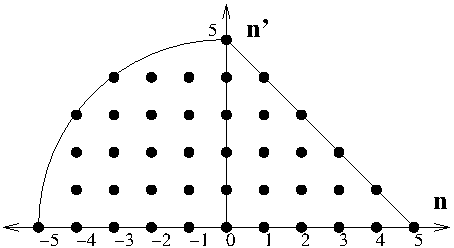
\includegraphics{wedge}
  \caption{A graph of the solutions to the Wedge schema}
  \label{fig:wedge}
\end{figure}

\begin{zsection}
  \SECTION wedge \parents standard\_toolkit
\end{zsection}
\begin{zed}
  State == [n: \negate 10 \upto 10] \\
  Wedge == [\Delta State | n*n + n'*n' \leq 25; n + n' \leq 5; 0 \leq n']
\end{zed}

\subsection{Positive Tests}

The first kind of testing we want to do is positive tests to check
that an operation has a desired input-output behaviour.  When
specifying tests, it is usual to specify the expected output
values as well as the input values, so we write all the inputs and
output values as a Z binding and use a membership test.  Here are two
examples that test the non-deterministic output behaviour of Wedge
when the input $n$ is zero.

\begin{zsection}
  \SECTION wedgeTest \parents wedge
\end{zsection}

\begin{theorem}{Wedge0Gives0}
  \vdash? ~ \lblot n==0, n'==0 \rblot \in Wedge
\end{theorem}
\vspace{-5ex}
\begin{theorem}{Wedge0Gives5}
  \vdash? ~ \lblot n==0, n'==5 \rblot \in Wedge
\end{theorem}

Note that since 2007, the Z standard requires conjectures
to be written within a \LaTeX\ \emph{theorem} environment, and allows
each conjecture to be given a name.  Our naming convention for tests
is that the name of a test should start with the name of the operation
being tested, followed by some phrase that expresses the essential
property of the test.

An alternative style of writing a suite of positive tests is to
name each test tuple, group the tuples into a set, and then test
them using a single subset conjecture.

\begin{zed}
  Wedge0Gives0 == \lblot n==0, n'==0 \rblot \\
  Wedge0Gives5 == \lblot n==0, n'==5 \rblot
\end{zed}

\begin{theorem}{WedgePos}
  \vdash? ~ \{Wedge0Gives0, Wedge0Gives5\} \subseteq Wedge
\end{theorem}


\subsection{Negative Tests}

It is also useful to perform \emph{negative} tests to validate an
operation.  For example, we may want to check that an input value is
outside the precondition of the operation, or check that a certain output
can never be produced by the operation.  The idea is to validate the
specification by showing that its behaviour is squeezed in between the set
of positive tests and the set of negative tests.  The more positive and
negative tests that we design, the more sure we can be that we have
specified the desired behaviour, rather than allowing too many or too few
behaviours.

We can write negative tests using a negated membership test ($test
\notin Op$) or, equivalently, we can test that the tuple is a member
of the negated schema ($test \in \lnot Op$).  Our conjecture naming
convention is the same as for positive tests, but the phrase after the
operation name usually contains a negative word such as \emph{not} or
\emph{cannot} to emphasize that it is a negative test.

\begin{theorem}{Wedge0NotNeg}
  \vdash? ~ \lblot n==0, n'==\negate 1 \rblot \notin Wedge
\end{theorem}
\vspace{-5ex}
\begin{theorem}{Wedge0Not6}
  \vdash? ~ \lblot n==0, n'==6 \rblot \in \lnot Wedge
\end{theorem}

We can also test just the precondition of the operation.
%% Note: ZLive cannot evaluate this if the type of x is any integer
%% because it requires enumerating pre Wedge, and then there is no
%% lower bound on $n'$.
\begin{theorem}{WedgePreNot6}
  \vdash? ~ \lblot n==6 \rblot \notin \pre Wedge
\end{theorem}

As we did for positive tests, we may also combine several negative tests
into a group.  In this case, our conjecture may be written as $tests
\subseteq \lnot Op$, or equivalently we may check that the intersection of
the negative test suite and the operation is empty, $tests \land Op =
\emptyset$.  The latter style is often more convenient, since it allows us
to write $tests$ using schema notation, and to omit variables that we are
not interested in (because the schema conjunction will expand the type of
$tests$ to match the type of $Op$).  For example, the following two negative
test suites check that 6 can never be an input for $Wedge$, and that 6 can
never be an output of $Wedge$.

\begin{theorem}{Wedge6Not}
  \vdash? ~ ([n==6] \land Wedge) = \emptyset
\end{theorem}
\vspace{-5ex}
\begin{theorem}{WedgeNot6}
  \vdash? ~ ([n'==6] \land Wedge) = \emptyset
\end{theorem}

It is sometimes convenient to write these kinds of negative test values
\emph{within} the operation schema (e.g., $[Wedge | n=6] = \emptyset$),
which can make the tests even more concise.


\subsection{Promoting Tests}

A heavily-used pattern in the POSIX Z specification is the use of
\emph{promotion} to lift the operations of one data type up to work on a
more complex data type.  It is useful to be able to promote the tests
of those operations as well.  To illustrate an elegant way of doing this,
we shall promote the $Wedge$ tests up to the following function space:

\begin{zsection}
  \SECTION manyStates \parents wedge
\end{zsection}

\begin{zed}
  ManyStates == [ states : \nat \fun \num ]
\end{zed}
\vspace{-5ex}
\begin{schema}{\Phi ManyStates}
  \Delta State \\
  \Delta ManyStates \\
  curr? : \nat
\where
  (curr? \mapsto n) \in states \\
  states' = states \oplus \{curr? \mapsto n'\}
\end{schema}

We promote the $Wedge$ operation up to the $ManyStates$ level simply by
conjoining $Wedge$ with the \emph{framing schema} $\Phi ManyStates$.
The effect is to apply the $Wedge$ operation to just the $curr?$ element of
the $states$ function.

\begin{zed}
  ManyWedge == \Phi ManyStates \land Wedge
\end{zed}


We use the same framing schema to promote the tests.  But to ensure
that all inputs of the promoted operation are given, we find it useful
to further instantiate the framing schema $\Phi ManyStates$, to obtain
a testing-oriented framing schema ($\Phi ManyStatesTest$) that also
specifies which $curr?$ input will be tested and an initial value for the
$states$ mapping.

\begin{zsection}
  \SECTION manyStatesTest \parents manyStates, wedgeTest
\end{zsection}
\vspace{-5ex}
\begin{zed}
  \Phi ManyStatesTest ==
    [\Phi ManyStates; curr? == 1 | states = \{0 \mapsto 3, 1 \mapsto n\}]
\end{zed}
\vspace{-5ex}
%% NOTE: this fails if State contains x, because of a scoping
%% error in the unfolding or in the translation to FlatPreds.
%% Probably an 'x' in the ZLive preprocess rules gets accidentally
%% bound to the 'x' from the State schema.
\begin{theorem}{ManyWedgePos}
  \vdash? ~ (\{Wedge0Gives0, Wedge0Gives5\} \land \Phi ManyStatesTest)
      \subseteq ManyWedge
\end{theorem}

In fact, this style of promoted test theorem will always be true,
because for any test suite $OpTests$ of an operation $Op$,
and any promoted operation defined as $Op_P == Op \land \Phi P$,
it is true that:
\[
   (OpTests \subseteq Op) \land (\Phi PTests \subseteq \Phi P)
   \implies (OpTests \land \Phi PTests \subseteq Op_P)
\]

\textbf{Proof:} follows from the monotonicity of $\subseteq$ and schema
conjunction. $\QED$

However, there is a possibility that some of the promoted tests
might be inconsistent with the framing schema (either $\Phi P$ or $\Phi
PTests$), which would mean that the set $OpTests \land \Phi PTests$
would be empty or smaller than our original set of tests $Optests$.
If we want to check that all of the original tests can be promoted without
being lost, we can check the conjecture
$(\Phi PTests \project OpTests) = Optests$.
%% ZLive does not correctly implement equality of sets of bindings yet.
%\begin{theorem}{AllTestsPromoted}
%\vdash? ~ (\Phi ManyStatesTest \project \{Wedge0Gives0, Wedge0Gives5\})
%            = \{Wedge0Gives0, Wedge0Gives5\}
%\end{theorem}

If this mass-promotion test fails, we may want to check each promoted test
vector $v \in Optests$ separately.  To do this, we can define the promoted
vector as $pv == (\mu \Phi PTests \land \{v\})$, and then we can test
$pv \in Op_P$.
%% ZLive gives a 'InclDecl not unfolded' error on this, because
%% the \mu \Phi ManyStatesTest is not fully unfolded yet.
%\begin{zed}
%  pv == (\mu \Phi ManyStatesTest \land \{Wedge0Gives0\})
%\end{zed}
%\begin{theorem}{ManyWedge0Gives0}
%  \vdash? ~ pv \in ManyWedge
%\end{theorem}


%%%%%%%%%%%%%%%%%%%%%%%%%%%%%%%%%%%%%%%%%%%%%%%%%%%%%%%%%%%%%%%%%%%%%%
\section{The ZLive Animator}\label{sect:zlive}
%%%%%%%%%%%%%%%%%%%%%%%%%%%%%%%%%%%%%%%%%%%%%%%%%%%%%%%%%%%%%%%%%%%%%%

One of the tools available in the CZT system is the ZLive animator.
It is the successor to the Jaza animator for Z~\cite{utting:jaza},
and its command line interface is largely backwards compatible with that of
Jaza.  However, the animation algorithm of ZLive is quite different and
more general.  It is based on an extension of the \emph{Z mode} system
developed at Melbourne University by Winikoff and
others~\cite{kazmierczak:animation98,winikoff:modes-subtypes98}.

When an expression or predicate is evaluated in ZLive, it is
parsed and typechecked, and then unfolded and simplified using
the \emph{transformation rules} system of CZT~\cite{utting:rules07}.
This unfolds schema operators, expands definitions and performs a
variety of simplifications.  For example, the test $\lblot n==0, n'==0
\rblot \in Wedge$ is unfolded to:
\[
  \lblot n == 0 , n' == 0 \rblot \in
 [ n :~\negate 10 \upto 10; n' :~\negate 10 \upto 10 | \\
   \t5 n * n + n' * n'  \leq 25; n + n' \leq 5; 0 \leq n' ]
\]

The resulting term is then translated into a sequence of primitive
relations, each of which corresponds to a single Z operator.
For example, the term $n * n + n' * n'  \leq 25$ is
translated into a sequence of four relations:
\[
\begin{array}{l@{\quad}l}
   FlatMult(n, n, tmp1),       & //~ n * n = tmp1 \\
   FlatMult(n', n', tmp2),     & //~ n' * n' = tmp2 \\
   FlatPlus(tmp1, tmp2, tmp3), & //~ tmp1 + tmp2 = tmp3 \\
   FlatLessThanEq(tmp3, 25)    & //~ tmp3 \leq 25
\end{array}
\]

ZLive next performs a bounds analysis phase, which does a fixpoint
calculation to infer conservative lower and upper bounds for each
integer variable, bounds on the size and contents of sets, and
aliasing between variables.  This infers that $n \in \negate 10 \upto
5$ and $n' \in 0 \upto 10$.

The last analysis phase attempts to reorder the sequence of primitive
$Flat\ldots$ relations into an efficient computation order.  Each of
the relations can be executed in one or more \emph{modes}.  A mode
determines whether each parameter is an input or an output.  In
addition, ZLive estimates the expected number of results for each
mode.  For example, the mode IIO:1 for $FlatPlus(x,y,z)$ means that
$x$ and $y$ are inputs and $z$ is an output (with one result
expected), while mode III:0.6 means they are all inputs and there is a
60\% probability of getting a result.  The reordering algorithm gives
preference to modes that have a small number of expected results,
which means that filter predicates are moved as near to the front as
possible, which reduces the search space.

Finally, ZLive enumerates all possible results via a depth-first
backtracking search of all the solutions generated by the sorted sequence.
However, for membership tests such as $A \in S$, where $A$ is a known
value and $S$ is a set comprehension, it substitutes the value of $A$
into the set comprehension for $S$ and then checks whether the set is
empty or not -- this avoids generating all of $S$.

ZLive can usually evaluate expressions that range over finite sets
only, and can sometimes handle expressions that contain a mixture of
finite and infinite sets.  So it is a useful tool for checking the
correctness of tests, and can sometimes be used to generate one
or all solutions of a partially specified test or schema.


%%%%%%%%%%%%%%%%%%%%%%%%%%%%%%%%%%%%%%%%%%%%%%%%%%%%%%%%%%%%%%%%%%%%%%
\section{POSIX Standardized}\label{sect:posix}
%%%%%%%%%%%%%%%%%%%%%%%%%%%%%%%%%%%%%%%%%%%%%%%%%%%%%%%%%%%%%%%%%%%%%%

In this section, we briefly describe the refactored POSIX specification.
The main change was to break up the original specification into sections.
Figure~\ref{fig:sects} shows the structure of the resulting Z
sections, using a notation similar to a UML class diagram.  Each box
represents a Z section, and the three parts within each box show the
name of the section, the main variables within the state schema of
that definition, and the names of its operation schemas (we omit Init
schemas and auxiliary schemas).  We also added a state schema and
initialization schema to some of the sections (e.g., the $ds$ section)
and made several naming changes so that the specification follows the
usual Z sequential style more closely.

\begin{figure}[htbp]
\newcommand{\DIVIDER}{\vspace{0.5ex} \hrule \vspace{1ex}}
\newcommand{\FATDIVIDER}{\vspace{1ex} \hrule \vspace{1.5ex}}
\newcommand{\SECTNAME}[2]{\hfil\hfil\hfil\textbf{#1}\hfil\emph{(#2)}}
  \centering
  \setlength{\unitlength}{0.9cm}
  \begin{picture}(13,20)
%
  \put(1,18){\framebox(8,1){\parbox{6\unitlength}{
        \hfil \textbf{standard\_toolkit} \hfil
    }}}
  \put(5,17){\vector(0,1){1}}
  \put(1,15){\framebox(8,2){\parbox{8\unitlength}{
        \SECTNAME{ds}{Data System}
        \DIVIDER
        ~$FILE == \seq BYTE$ \\ \hbox{}
        ~$file : FILE$
        \DIVIDER
        $~readFILE, writeFILE$
    }}}
  \put(5,14){\vector(0,1){1}}
  \put(1,12){\framebox(8,2){\parbox{8\unitlength}{
        \SECTNAME{ss}{Storage System}
        \FATDIVIDER
        ~$fstore : FID \pfun FILE$
        \FATDIVIDER
        $~createSS, destroySS, readSS, writeSS$
    }}}
  \put(5,11){\vector(0,1){1}}
  \put(1,9){\framebox(8,2){\parbox{8\unitlength}{
        \SECTNAME{cs}{Channel System}
        \FATDIVIDER
        ~$cstore : CID \pfun CHAN$
        \FATDIVIDER
        $~openCS, closeCS$
    }}}
  \put(5,8){\vector(0,1){1}}
  \put(1,6){\framebox(8,2){\parbox{8\unitlength}{
        \SECTNAME{as}{Access System}
        \FATDIVIDER
        ~$SS; CS$
        \FATDIVIDER
        $~readAS, writeAS, seekAS$
    }}}
  \put(5,5){\vector(0,1){1}}
  \put(1,3){\framebox(8,2){\parbox{8\unitlength}{
        \SECTNAME{ns}{Name System}
        \FATDIVIDER
        ~$nstore : NAME \pfun FID$
        \FATDIVIDER
        $~createNS, lookupNS, destroyNS, lsNS$
    }}}
  \put(5,2){\vector(0,1){1}}
  \put(1,0){\framebox(8,2){\parbox{8\unitlength}{
        \SECTNAME{fs}{File System}
        \DIVIDER
        ~$SS; CS; NS; usedfids : \power FID$
        \DIVIDER
        $~createFS, openFS, readFS, writeFS, closeFS,$ \\
        \hbox{}$~unlinkFS0, destroyFS, linkFS, moveFS$
    }}}
%
% Now add the unit test sections
% dstest has ds as a parent
  \put(12,15){\vector(-3,1){3}}
  \put(10,14){\framebox(4,1){\parbox{4\unitlength}{
        \hfil \textbf{dstest} \hfil
    }}}
% sstest has dstest and ss as parents
  \put(12,12){\vector(-3,1){3}}
  \put(12,12){\vector(0,1){2}}
  \put(10,11){\framebox(4,1){\parbox{4\unitlength}{
        \hfil \textbf{sstest} \hfil
    }}}
% cstest has sstest and cs as parents
  \put(12,9){\vector(-3,1){3}}
  \put(12,9){\vector(0,1){2}}
  \put(10,8){\framebox(4,1){\parbox{4\unitlength}{
        \hfil \textbf{$\cdots$} \hfil
    }}}
%
  \end{picture}
  \caption{Overview of Z Sections in the Refactored POSIX Specification}
  \label{fig:sects}
\end{figure}

\input{ds.zed}

%%%%%%%%%%%%%%%%%%%%%%%%%%%%%%%%%%%%%%%%%%%%%%%%%%%%%%%%%%%%%%%%%%%%%%
\section{Testing the DS Specification}\label{sect:ds}
%%%%%%%%%%%%%%%%%%%%%%%%%%%%%%%%%%%%%%%%%%%%%%%%%%%%%%%%%%%%%%%%%%%%%%


\input{dstest.zed}


%%%%%%%%%%%%%%%%%%%%%%%%%%%%%%%%%%%%%%%%%%%%%%%%%%%%%%%%%%%%%%%%%%%%%%
\section{Testing the SS Specification}\label{sect:ss}
%%%%%%%%%%%%%%%%%%%%%%%%%%%%%%%%%%%%%%%%%%%%%%%%%%%%%%%%%%%%%%%%%%%%%%

The storage system is reponsible for mapping \emph{file identifiers}
$FID$ to file contents.  While testing, we instantiate FID to
naturals, so test values are easier to write.

\begin{zsection}
  \SECTION ss \parents ds
\end{zsection}
\vskip -4ex
\begin{zed}
%  [FID]
  FID == \nat \\
  SS == [ fstore : FID \pfun FILE ]
\end{zed}

The $ss$ section then defines $createSS$ and $destroySS$ operations,
plus the following framing schema, which is used to promote $readFILE$
and $writeFILE$.

\begin{schema}{\Phi SS}
  \Delta SS;  ~
  \Delta DS;  ~
  fid? : FID
\where
  fid? \in \dom fstore \\
  file = fstore(fid?) \\
  fstore' = fstore \oplus \{ fid? \mapsto file' \}
\end{schema}
\vskip -2ex
\begin{zed}
  readSS == (\Phi SS \land readFILE) \hide (file, file') \\
%  writeSS == (\Phi SS \land writeFILE) \hide (file, file')
\end{zed}
\vskip -2ex

\input{sstest.zed}


%%%%%%%%%%%%%%%%%%%%%%%%%%%%%%%%%%%%%%%%%%%%%%%%%%%%%%%%%%%%%%%%%%%%%%
\section{Conclusions}\label{sect:conclusions}
%%%%%%%%%%%%%%%%%%%%%%%%%%%%%%%%%%%%%%%%%%%%%%%%%%%%%%%%%%%%%%%%%%%%%%

In this paper, we have proposed a framework for unit testing Z
specifications.  The framework uses the sections and conjectures of
the Z standard to allow various kinds of validation tests to be
expressed in an elegant and concise style.  The ability to promote a
large set of tests in a single expression makes it practical to
develop multiple layers of tests, matching the layers of the
specification.  Testing is a useful validation technique for
specifications, especially when the execution of the tests can be
automated, as we have done with ZLive.  We believe that most Z
specifications should include validation unit tests in this style.

We plan to add a \texttt{unittest} command to ZLive that executes all the
unit tests in all the sections whose names end with `Test'.  This will
make it easy to rerun all unit tests after each modification of a
specification, so will support regression testing during development
of Z specifications.  It would also be useful if ZLive measured structural
coverage metrics of the operation schemas during testing, so that we
can see what level of, say, branch coverage (each predicate evaluating to
true and to false) our test suite obtains.

Our style of unit testing is quite complementary to the specification
validation facilities of ProB/ProZ~\cite{leuschel:prob08}, because we
focus on unit testing of each individual operation schema using a
manually designed test suite, while ProB focusses on automatic testing
of sequences of operations, and tests only a few input values of each
operation.  The goal of our unit testing is to test the input-output
functionality of each operation, while the main goal of ProB is to try to
validate several standard system properties such as absence of deadlock and
preservation of invariants.

The refactored Z specification of POSIX, and our simple test suite,
may be a useful starting point for other researchers who want to work
on refinement or proofs about the POSIX case study.  It is available
from the CZT sourceforge website~\cite{CZT}.  Interestingly, the
original POSIX specification did include several examples that used
test values to illustrate some of the operations, but those examples
were written within the English commentary, so were not even
typechecked, let alone proved correct.  Our unit tests are more
systematic and are formalized so that they can be checked
automatically by an animator like ZLive.


%
% ---- Bibliography ----
%
\bibliographystyle{alpha}
\bibliography{posix}
%\begin{thebibliography}{5}
%
%\bibitem {clarke}
%\end{thebibliography}
\end{document}
